\documentclass[aspectratio=169]{beamer}
\usepackage{amsmath}
\usepackage{amssymb}
\usepackage{tikz}
\usepackage{xcolor}
\usetikzlibrary{shapes,backgrounds,patterns}

\usepackage{pgfplots}
\pgfplotsset{compat=1.18, legend cell align=left}
\usetikzlibrary{arrows.meta,decorations.pathreplacing,calc,positioning}
\usepackage{booktabs}
\usepackage{pifont}
\usepgfplotslibrary{fillbetween}

% royalblue isn't a base xcolor name, so define it first (this is the default accent)
\definecolor{royalblue}{RGB}{65,105,225}

% ============================================================
%  ACCENT COLOR: change ONE line below to switch the theme
%  Choose one of: royalblue , red , black
% ============================================================
\colorlet{accent}{royalblue}
% \colorlet{accent}{red}
% \colorlet{accent}{black}
% ============================================================

% colorblind-safe, high-contrast second color (Okabe-Ito vermillion)
\definecolor{hl}{RGB}{213,94,0}

\usetheme{default}
\setbeamercolor{background canvas}{bg=white}
\setbeamercolor{normal text}{fg=black}
\setbeamercolor{structure}{fg=accent}
\setbeamercolor{frametitle}{fg=accent,bg=white}
\setbeamercolor{title}{fg=accent}
\setbeamercolor{section in toc}{fg=black}
\setbeamercolor{block title}{fg=black,bg=gray!10}
\setbeamercolor{block body}{fg=black,bg=gray!5}
\setbeamercolor{block title example}{fg=black,bg=green!10}
\setbeamercolor{block body example}{fg=black,bg=green!5}
\setbeamercolor{block title alerted}{fg=black,bg=red!10}
\setbeamercolor{block body alerted}{fg=black,bg=red!5}

\setbeamertemplate{navigation symbols}{}
\setbeamertemplate{footline}{
    \hfill\makebox[5pt]{%
        \scriptsize\insertframenumber}
    \hspace*{2em}
    \vspace{0.5cm}
}

\newcommand{\cbox}[2]{\colorbox{#1}{\ensuremath{\displaystyle #2}}}

\pgfplotsset{
  miniplot/.style={
    width=4.0cm, height=3.0cm,
    axis lines=middle, xtick=\empty, ytick=\empty,
    samples=120, thick, clip=true
  }
}

\definecolor{gr}{RGB}{0,158,115}


% curve and helpers for the three-rule picture
\pgfmathdeclarefunction{fc}{1}{\pgfmathparse{0.55+1.25*sin(deg(0.85*#1))}}
\pgfmathdeclarefunction{gc}{1}{\pgfmathparse{0.55+0.3*sin(deg(#1))+1.1*exp(-4*(#1-2.6)^2)}}
\pgfplotsset{
  rule2/.style={
    width=5.4cm, height=3.6cm, axis lines=middle, xmin=0, xmax=4.3, ymin=0, ymax=1.95,
    xtick=\empty, ytick=\empty, thick, clip=false,
    title style={font=\small}
  }
}
\pgfplotsset{
  rule/.style={
    width=5.4cm, height=4.2cm, axis lines=middle, xmin=0, xmax=4.3, ymin=0, ymax=1.95,
    xtick=\empty, ytick=\empty, thick, clip=false, samples=100,
    title style={font=\small}
  }
}

\pgfplotsset{
  rev/.style={
    width=4.9cm, height=3.1cm, axis lines=middle, xmin=0, xmax=4.3, ymin=0, ymax=1.95,
    xtick=\empty, ytick=\empty, thick, clip=false,
    title style={font=\small, yshift=-4pt, text depth=0pt, text height=1.6ex}
  }
}

\title{The Discrete Fourier Transform}
\subtitle{Finding the frequencies hidden in a signal}
\author{Sharareh Sayyad}
\institute{Washington State University}
\date{\today}

\begin{document}
\frame{\titlepage}

% ------------------------------------------------------------
\begin{frame}{Can you taste the recipe?}
\begin{columns}[c]
\begin{column}{0.52\textwidth}
\centering
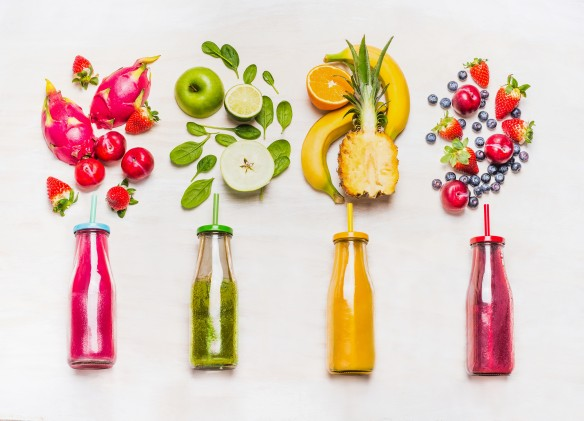
\includegraphics[width=\textwidth]{smoothies.jpg}
\end{column}
\begin{column}{0.46\textwidth}
\small
Each smoothie is a \textbf{mix} of fruits

\vspace{0.4em}
We only get the \textbf{drink}, not the fruits

\vspace{0.4em}
\textbf{Question:} Which fruits are in it, and how much of each?

\vspace{1.0em}
\footnotesize
\begin{tabular}{@{}l@{\ \ $\leftrightarrow$\ \ }l@{}}
A fruit & A pure wave (one frequency)\\[2pt]
The smoothie & The signal we measure\\[2pt]
The recipe & The frequencies and amounts
\end{tabular}

\vspace{1.0em}
\small
The \textbf{Fourier transform} un-mixes a signal
\end{column}
\end{columns}

\vspace{0.8em}
\raggedright
\tiny Image from \href{https://methodsblog.com/2016/12/15/fourier-analysis/}{\texttt{https://methodsblog.com/2016/12/15/fourier-analysis/}}
\end{frame}

% ------------------------------------------------------------
\begin{frame}{The smoothie problem}
\centering
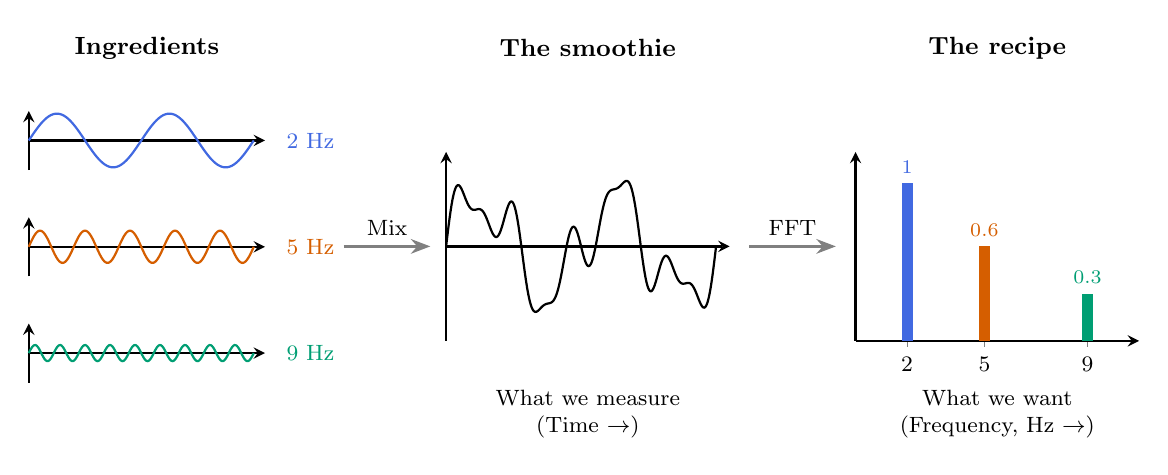
\begin{tikzpicture}
\pgfplotsset{
  ing/.style={scale only axis, width=3.0cm, height=0.75cm, axis lines=middle,
    xtick=\empty, ytick=\empty, xmin=0, xmax=1.05, ymin=-1.1, ymax=1.1, thick, clip=false, samples=200}}

% --- column 1: the ingredients ---
\node[font=\small\bfseries] at (1.5,1.55) {Ingredients};
\begin{axis}[ing, at={(0,0)}]
\addplot[accent, domain=0:1] {sin(deg(2*pi*2*x))};
\end{axis}
\node[font=\footnotesize, accent, anchor=west] at (3.15,0.375) {2 Hz};
\begin{axis}[ing, at={(0,-1.35cm)}]
\addplot[hl, domain=0:1] {0.6*sin(deg(2*pi*5*x))};
\end{axis}
\node[font=\footnotesize, hl, anchor=west] at (3.15,-0.975) {5 Hz};
\begin{axis}[ing, at={(0,-2.7cm)}]
\addplot[gr, domain=0:1] {0.3*sin(deg(2*pi*9*x))};
\end{axis}
\node[font=\footnotesize, gr, anchor=west] at (3.15,-2.325) {9 Hz};

% arrow: mix
\draw[-{Stealth[length=7pt]}, very thick, gray] (4.0,-0.97) -- (5.1,-0.97) node[midway, above, font=\footnotesize, black] {Mix};

% --- column 2: the smoothie ---
\node[font=\small\bfseries] at (7.1,1.55) {The smoothie};
\begin{axis}[scale only axis, width=3.6cm, height=2.4cm, axis lines=middle, xtick=\empty, ytick=\empty,
  xmin=0, xmax=1.05, ymin=-2.0, ymax=2.0, thick, clip=false, samples=300, at={(5.3cm,-2.17cm)}]
\addplot[black, domain=0:1] {sin(deg(2*pi*2*x)) + 0.6*sin(deg(2*pi*5*x)) + 0.3*sin(deg(2*pi*9*x))};
\end{axis}
\node[font=\footnotesize, align=center] at (7.1,-3.1) {What we measure\\(Time $\to$)};

% arrow: FFT
\draw[-{Stealth[length=7pt]}, very thick, gray] (9.15,-0.97) -- (10.25,-0.97) node[midway, above, font=\footnotesize, black] {FFT};

% --- column 3: the recipe ---
\node[font=\small\bfseries] at (12.3,1.55) {The recipe};
\begin{axis}[scale only axis, width=3.6cm, height=2.4cm, axis lines=left, xmin=0, xmax=11, ymin=0, ymax=1.2,
  xtick={2,5,9}, ytick=\empty, ticklabel style={font=\footnotesize}, thick, clip=false, at={(10.5cm,-2.17cm)}]
\draw[accent, line width=4pt] (axis cs:2,0) -- (axis cs:2,1);
\draw[hl, line width=4pt] (axis cs:5,0) -- (axis cs:5,0.6);
\draw[gr, line width=4pt] (axis cs:9,0) -- (axis cs:9,0.3);
\node[font=\scriptsize, accent, above] at (axis cs:2,1) {1};
\node[font=\scriptsize, hl, above] at (axis cs:5,0.6) {0.6};
\node[font=\scriptsize, gr, above] at (axis cs:9,0.3) {0.3};
\end{axis}
\node[font=\footnotesize, align=center] at (12.3,-3.1) {What we want\\(Frequency, Hz $\to$)};
\end{tikzpicture}

\vspace{0.8em}
\small
$x(t) = \textcolor{accent}{1\cdot\sin(2\pi\cdot 2\,t)} + \textcolor{hl}{0.6\cdot\sin(2\pi\cdot 5\,t)} + \textcolor{gr}{0.3\cdot\sin(2\pi\cdot 9\,t)}$

\vspace{0.8em}
\cbox{accent!12}{\text{Goal: Given only the smoothie } x(t)\text{, find which frequencies are in it and how much of each}}
\end{frame}

% ------------------------------------------------------------
\begin{frame}{What about noise?}
\centering
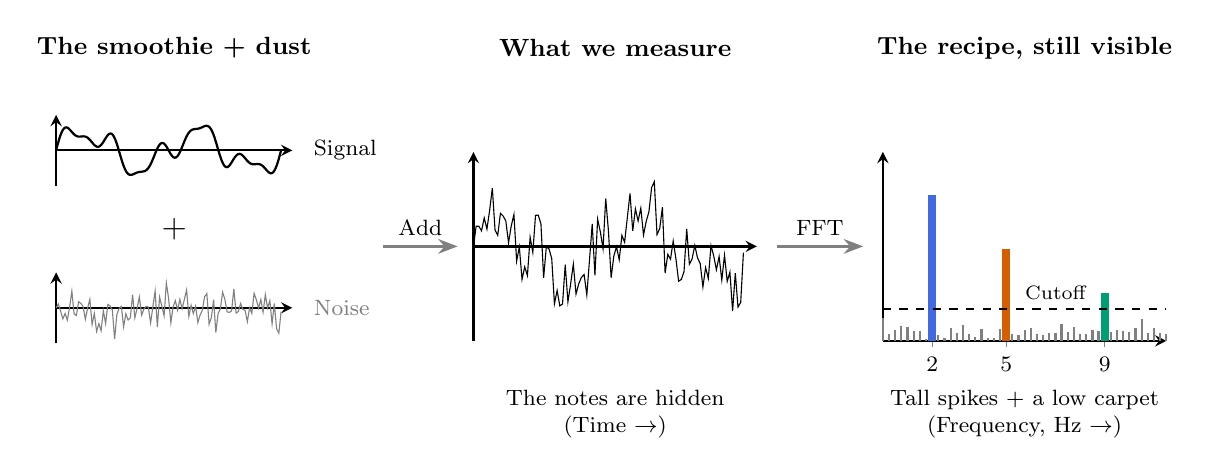
\begin{tikzpicture}
\pgfplotsset{
  ing/.style={scale only axis, width=3.0cm, height=0.9cm, axis lines=middle,
    xtick=\empty, ytick=\empty, xmin=0, xmax=1.05, ymin=-2.0, ymax=2.0, thick, clip=false, samples=200}}

% --- column 1: clean signal + noise ---
\node[font=\small\bfseries] at (1.5,1.55) {The smoothie + dust};
\begin{axis}[ing, at={(0,-0.2cm)}]
\addplot[black, domain=0:1] {sin(deg(2*pi*2*x)) + 0.6*sin(deg(2*pi*5*x)) + 0.3*sin(deg(2*pi*9*x))};
\end{axis}
\node[font=\footnotesize, anchor=west] at (3.15,0.25) {Signal};
\node[font=\large] at (1.5,-0.75) {$+$};
\begin{axis}[ing, at={(0,-2.2cm)}]
\addplot[gray, thin] coordinates {(0.000,0.001) (0.010,0.209) (0.020,-0.192) (0.030,-0.623) (0.040,-0.318) (0.050,-0.694) (0.060,0.042) (0.070,0.938) (0.080,-0.345) (0.090,-0.434) (0.100,0.343) (0.110,0.250) (0.120,0.074) (0.130,-0.651) (0.140,-0.020) (0.150,0.487) (0.160,-0.941) (0.170,-0.320) (0.180,-1.331) (0.190,-0.903) (0.200,-1.289) (0.210,-0.165) (0.220,-0.887) (0.230,0.190) (0.240,0.110) (0.250,-0.131) (0.260,-1.762) (0.270,-0.377) (0.280,-0.034) (0.290,0.079) (0.300,-1.071) (0.310,-0.334) (0.320,-0.685) (0.330,-0.566) (0.340,0.743) (0.350,-0.565) (0.360,-0.023) (0.370,0.619) (0.380,-0.409) (0.390,-0.078) (0.400,0.077) (0.410,0.045) (0.420,-0.858) (0.430,0.053) (0.440,0.951) (0.450,-1.083) (0.460,0.602) (0.470,0.084) (0.480,-0.449) (0.490,1.400) (0.500,0.534) (0.510,-0.840) (0.520,0.052) (0.530,0.404) (0.540,-0.132) (0.550,0.478) (0.560,-0.047) (0.570,0.467) (0.580,1.007) (0.590,-0.473) (0.600,0.142) (0.610,-0.324) (0.620,0.089) (0.630,-0.831) (0.640,-0.406) (0.650,-0.137) (0.660,0.629) (0.670,0.802) (0.680,-0.926) (0.690,-0.556) (0.700,0.453) (0.710,-1.395) (0.720,-0.324) (0.730,-0.068) (0.740,0.880) (0.750,0.483) (0.760,-0.229) (0.770,-0.258) (0.780,-0.175) (0.790,1.066) (0.800,-0.300) (0.810,-0.213) (0.820,0.247) (0.830,-0.085) (0.840,-0.138) (0.850,-0.780) (0.860,-0.008) (0.870,-0.311) (0.880,0.816) (0.890,0.457) (0.900,-0.017) (0.910,0.468) (0.920,-0.238) (0.930,0.736) (0.940,-0.004) (0.950,0.408) (0.960,-0.904) (0.970,0.243) (0.980,-1.182) (0.990,-1.425) (1.000,-0.213)};
\end{axis}
\node[font=\footnotesize, gray, anchor=west] at (3.15,-1.75) {Noise};

% arrow: add
\draw[-{Stealth[length=7pt]}, very thick, gray] (4.15,-0.97) -- (5.1,-0.97) node[midway, above, font=\footnotesize, black] {Add};

% --- column 2: what we measure ---
\node[font=\small\bfseries] at (7.1,1.55) {What we measure};
\begin{axis}[scale only axis, width=3.6cm, height=2.4cm, axis lines=middle, xtick=\empty, ytick=\empty,
  xmin=0, xmax=1.05, ymin=-3.2, ymax=3.2, thick, clip=false, at={(5.3cm,-2.17cm)}]
\addplot[black, thin] coordinates {(0.000,0.001) (0.010,0.681) (0.020,0.681) (0.030,0.528) (0.040,0.965) (0.050,0.586) (0.060,1.223) (0.070,1.975) (0.080,0.558) (0.090,0.377) (0.100,1.118) (0.110,1.028) (0.120,0.864) (0.130,0.124) (0.140,0.691) (0.150,1.080) (0.160,-0.496) (0.170,-0.018) (0.180,-1.118) (0.190,-0.694) (0.200,-0.987) (0.210,0.311) (0.220,-0.204) (0.230,1.052) (0.240,1.059) (0.250,0.769) (0.260,-1.063) (0.270,-0.013) (0.280,-0.087) (0.290,-0.408) (0.300,-1.944) (0.310,-1.495) (0.320,-2.014) (0.330,-1.952) (0.340,-0.622) (0.350,-1.874) (0.360,-1.276) (0.370,-0.601) (0.380,-1.615) (0.390,-1.265) (0.400,-1.050) (0.410,-0.954) (0.420,-1.644) (0.430,-0.450) (0.440,0.763) (0.450,-0.978) (0.460,0.922) (0.470,0.498) (0.480,-0.074) (0.490,1.621) (0.500,0.534) (0.510,-1.060) (0.520,-0.323) (0.530,-0.011) (0.540,-0.452) (0.550,0.373) (0.560,0.142) (0.570,0.971) (0.580,1.793) (0.590,0.525) (0.600,1.270) (0.610,0.862) (0.620,1.295) (0.630,0.390) (0.640,0.848) (0.650,1.171) (0.660,1.994) (0.670,2.188) (0.680,0.402) (0.690,0.604) (0.700,1.326) (0.710,-0.907) (0.720,-0.271) (0.730,-0.433) (0.740,0.181) (0.750,-0.417) (0.760,-1.178) (0.770,-1.120) (0.780,-0.858) (0.790,0.591) (0.800,-0.602) (0.810,-0.421) (0.820,0.034) (0.830,-0.387) (0.840,-0.583) (0.850,-1.374) (0.860,-0.719) (0.870,-1.086) (0.880,0.026) (0.890,-0.321) (0.900,-0.792) (0.910,-0.343) (0.920,-1.140) (0.930,-0.301) (0.940,-1.184) (0.950,-0.872) (0.960,-2.187) (0.970,-0.908) (0.980,-2.055) (0.990,-1.896) (1.000,-0.213)};
\end{axis}
\node[font=\footnotesize, align=center] at (7.1,-3.1) {The notes are hidden\\(Time $\to$)};

% arrow: FFT
\draw[-{Stealth[length=7pt]}, very thick, gray] (9.15,-0.97) -- (10.25,-0.97) node[midway, above, font=\footnotesize, black] {FFT};

% --- column 3: the spectrum ---
\node[font=\small\bfseries] at (12.3,1.55) {The recipe, still visible};
\begin{axis}[scale only axis, width=3.6cm, height=2.4cm, axis lines=left, xmin=0, xmax=11.5, ymin=0, ymax=1.2,
  xtick={2,5,9}, ytick=\empty, ticklabel style={font=\footnotesize}, thick, clip=false, at={(10.5cm,-2.17cm)}]
\addplot[ycomb, gray, thick] coordinates {(0.000,0.148) (0.250,0.046) (0.500,0.069) (0.750,0.093) (1.000,0.086) (1.250,0.064) (1.500,0.063) (1.750,0.012) (2.000,0.929) (2.250,0.036) (2.500,0.021) (2.750,0.084) (3.000,0.048) (3.250,0.103) (3.500,0.042) (3.750,0.027) (4.000,0.078) (4.250,0.021) (4.500,0.018) (4.750,0.077) (5.000,0.583) (5.250,0.046) (5.500,0.035) (5.750,0.072) (6.000,0.079) (6.250,0.043) (6.500,0.040) (6.750,0.050) (7.000,0.049) (7.250,0.108) (7.500,0.058) (7.750,0.085) (8.000,0.046) (8.250,0.042) (8.500,0.071) (8.750,0.060) (9.000,0.305) (9.250,0.055) (9.500,0.067) (9.750,0.060) (10.000,0.058) (10.250,0.079) (10.500,0.142) (10.750,0.049) (11.000,0.079) (11.250,0.049) (11.500,0.043)};
\draw[accent, line width=3pt] (axis cs:2,0) -- (axis cs:2,0.929);
\draw[hl, line width=3pt] (axis cs:5,0) -- (axis cs:5,0.583);
\draw[gr, line width=3pt] (axis cs:9,0) -- (axis cs:9,0.305);
\draw[black, dashed] (axis cs:0,0.2) -- (axis cs:11.5,0.2);
\node[font=\scriptsize, anchor=south] at (axis cs:7,0.2) {Cutoff};
\end{axis}
\node[font=\footnotesize, align=center] at (12.3,-3.1) {Tall spikes + a low carpet\\(Frequency, Hz $\to$)};
\end{tikzpicture}

\vspace{0.4em}
\small
Noise is spread \textbf{thinly over all frequencies}, \ each note is \textbf{concentrated in one}

\vspace{0.3em}
\textbf{Denoise:} Keep the spikes above the cutoff, set the carpet to 0, transform back

\vspace{0.4em}
\cbox{hl!12}{\text{The notes stand out as long as each spike is taller than the noise carpet}}
\end{frame}

\end{document}
